% !TEX root = QlockToo.tex
% Kapitelvorlage

\section{Einleitung}
\label{sec:Einleitung}

\begin{figure}[t]
    \centering
    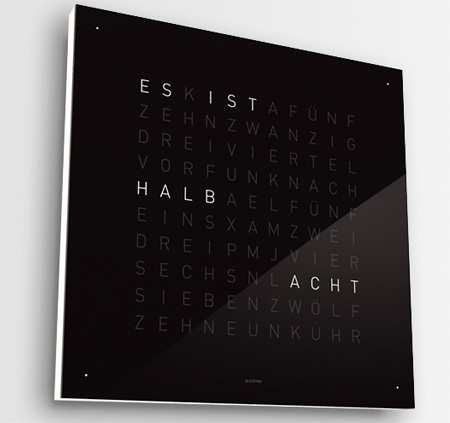
\includegraphics[width=9cm]{Abbildungen/qlocktwo-wand}
    \caption[ClockTwo]{CLOCKTWO CLASSIC}
    \label{fig:ClockTwo}
\end{figure}
%
 \begin{multicols}{2}
 In der heutigen Zeit steht neben der Funktionalität vieler Dinge ihr Design im Vordergrund. Bestes Beispiel ist die CLOCKTWO® der Biegert \&  Funk Manufacture GmbH \& Co. KG. Abbildung~\ref{fig:ClockTwo} zeigt die CLOCKTWO CLASSIC als Wand- oder Standuhr. %Die QLOCKTWO® ist ein international eingetragenes Markenzeichen, welches zudem durch internationale Patente und Designpatente geschützt ist. 
 Zeit in zeitlosem Design -   so bewirbt die Designmanufaktur die einzigartige Uhr.  Inspiriert durch diese außergewöhnliche Darstellung der Zeit in geschriebenen Worten, entsteht das Entwicklungs- und Fertigungskonzept einer elektronischen Wanduhr mit einer LED-Matrix. \textit{We can built a CLOCK, TOO.}
 \end{multicols}
 %
 \begin{figure}[h]
    \centering
    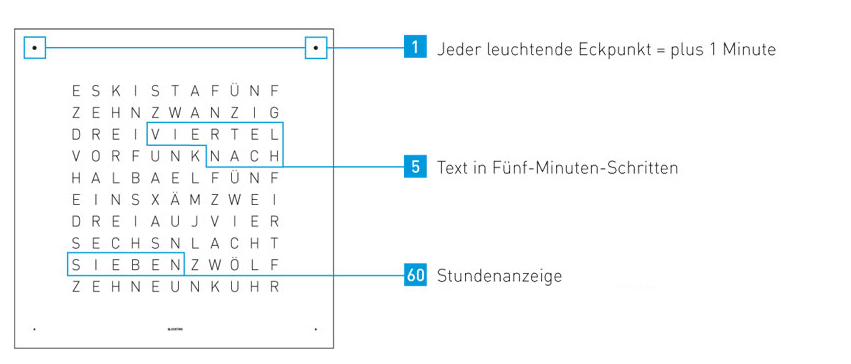
\includegraphics[width=13cm]{Abbildungen/Uhrzeit_Beispiel}
    \caption[Uhrzeit_Bspl]{Beispiel: 7 Uhr 17}
    \label{fig:Uhrzeit_Bspl}
\end{figure}
 %
 \begin{figure}[t]
    \centering
    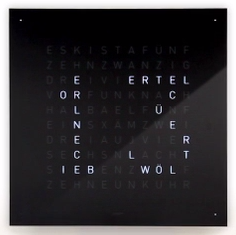
\includegraphics[width=7cm]{Abbildungen/Sekunden}
    \caption[Sekunden]{Darstellung der Sekunden}
    \label{fig:Sekunden}
\end{figure}
%
  \begin{multicols}{2}
Die Zeitanzeige erfolgt auf einer Buchstabenmatrix in Fünf-Minuten-Schritten, siehe Abbildung~\ref{fig:Uhrzeit_Bspl}. Die Worte werden durch Ausleuchten einer Buchstabenfolie auf einer Plexiglasscheibe durch LEDs abgebildet. Durch vier zusätzliche Leuchtpunkte in den Ecken der Uhr werden die Minuten zwischen den Intervallen angezeigt. Abbildung~\ref{fig:Sekunden} zeigt die Darstellung der Sekunden. Auf der kompletten Matrix kann ebenfalls die Raumtemperatur angezeigt werden. Die Umstellung erfolgt sowie die Auswahl weiterer Funktionen über seitliche Taster. Vor der Konzeption der Wortuhr steht die Programmierung einer Desktop-Software, welche den Testprozess der Algorithmen beschleunigt. Die Software ermöglicht zudem die Darstellung weiterer Unterprogramme. 
Bei der Konstruktion sowie die Fertigung des Uhrgehäuses werden Kaufteile mit Eigenproduktionen kombiniert, um dem äußeren Erscheinungsbild des Originals möglichst nah zu kommen und die Kosten gering zu halten. Die Entwicklung eines Elektronikkonzeptes ist  weiterer fundamentaler Bestandteil des Projektes.
\end{multicols}



